\section{Geant4シミュレーションによるテスト実験の再現}
製作したコーン型ライトガイドの集光性能を確認するため、Geant4シミュレーションによるプロトタイプ検出器の再現を行った。
コーン型ライトガイドの集光性能を確認することで、実機のシミュレーションにおいてより正確なシミュレーションを行うことができる。

\subsection{ジオメトリ}

\begin{figure}[htbp]
  \centering
  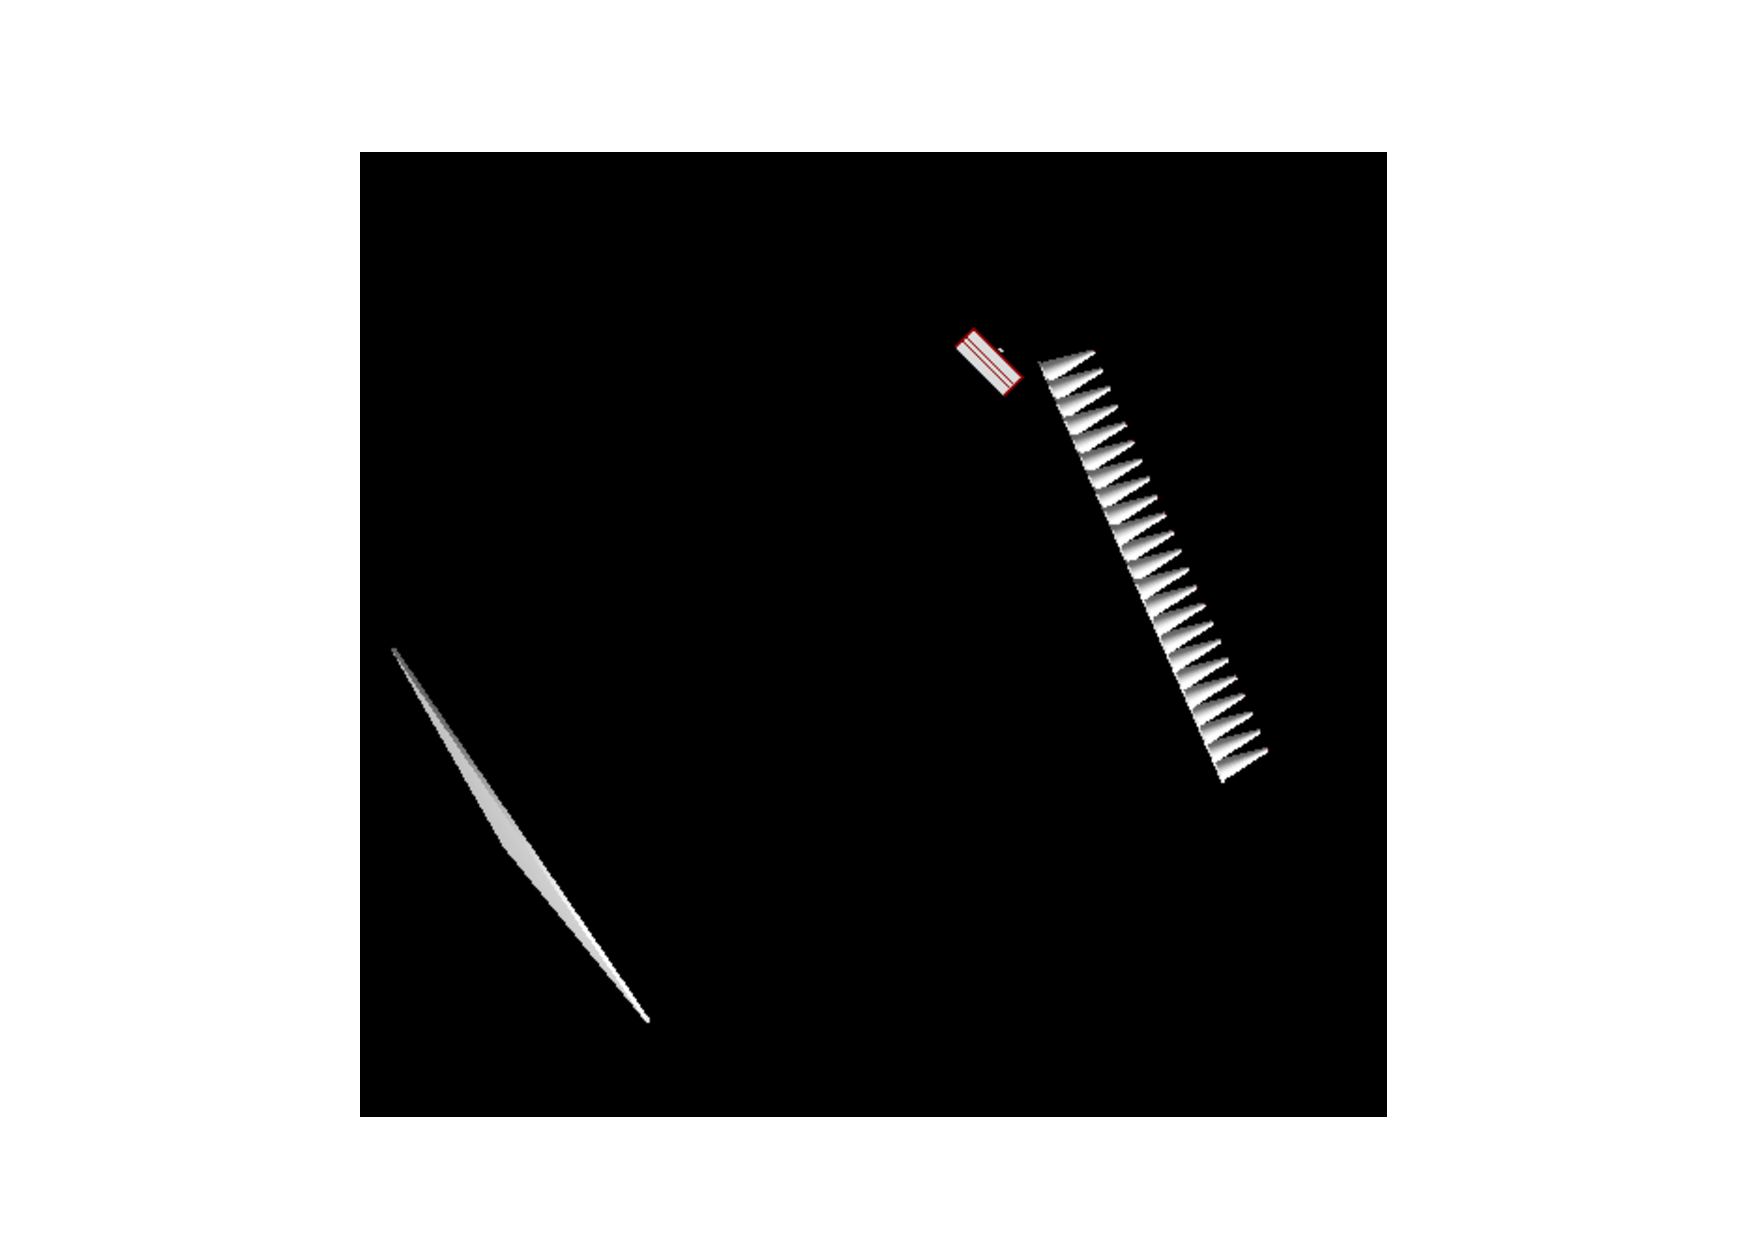
\includegraphics[width=10cm, page=1]{images/chapter4/ELPHsimulationSetup.pdf}
  \caption{テスト実験再現用シミュレーションのセットアップ。上から見た図。}
  \label{fig:ELPHsimulationSetup1}
\end{figure}

\subsection{エアロゲル}
エアロゲルはサイズ、屈折率、透過長、吸収長、をパラメータとして考慮した。
実験と同様に3つのエアロゲルを並べて厚さ$\SI{50}{mm}$とし、
表\ref{table:Aerogel}に示すエアロゲルの内、ビーム上流側から
TSA9-3、TSA10-3、TSATSA9-4の3つのパラメータを設定した。
屈折率は波長に依らず一定とし、透過長はレイリー散乱の波長の4乗に比例する関係を考慮して設定した。
吸収長は全てのエアロゲルで波長に依らず5500 mmとし、縦横のサイズは全て$\SI{146}{mm}\times\SI{146}{mm}$とした。

\subsection{球面鏡}
球面鏡は、曲率半径$2982 \si{mm}$、外径は$\SI{1009}{mm}\times\SI{1009}{mm}$とした。
反射率は、図\ref{fig:Al_reflection}を参考に波長依存性を考慮して設定した。

\subsection{MPPC}
MPPCは図\ref{fig:MPPCshape}を参考に、受光面を$\SI{6}{mm}(縦)\times\SI{6}{mm}(横)\times\SI{1.3}{mm}(厚さ)$のシリコンとし、
受光面の上に窓材として厚さ$\SI{4}{mm}$のシリコンを設定した。
受光面のシリコンは屈折率1.41、吸収長$\SI{0.001}{mm}$とした。

\begin{figure}
  \centering
  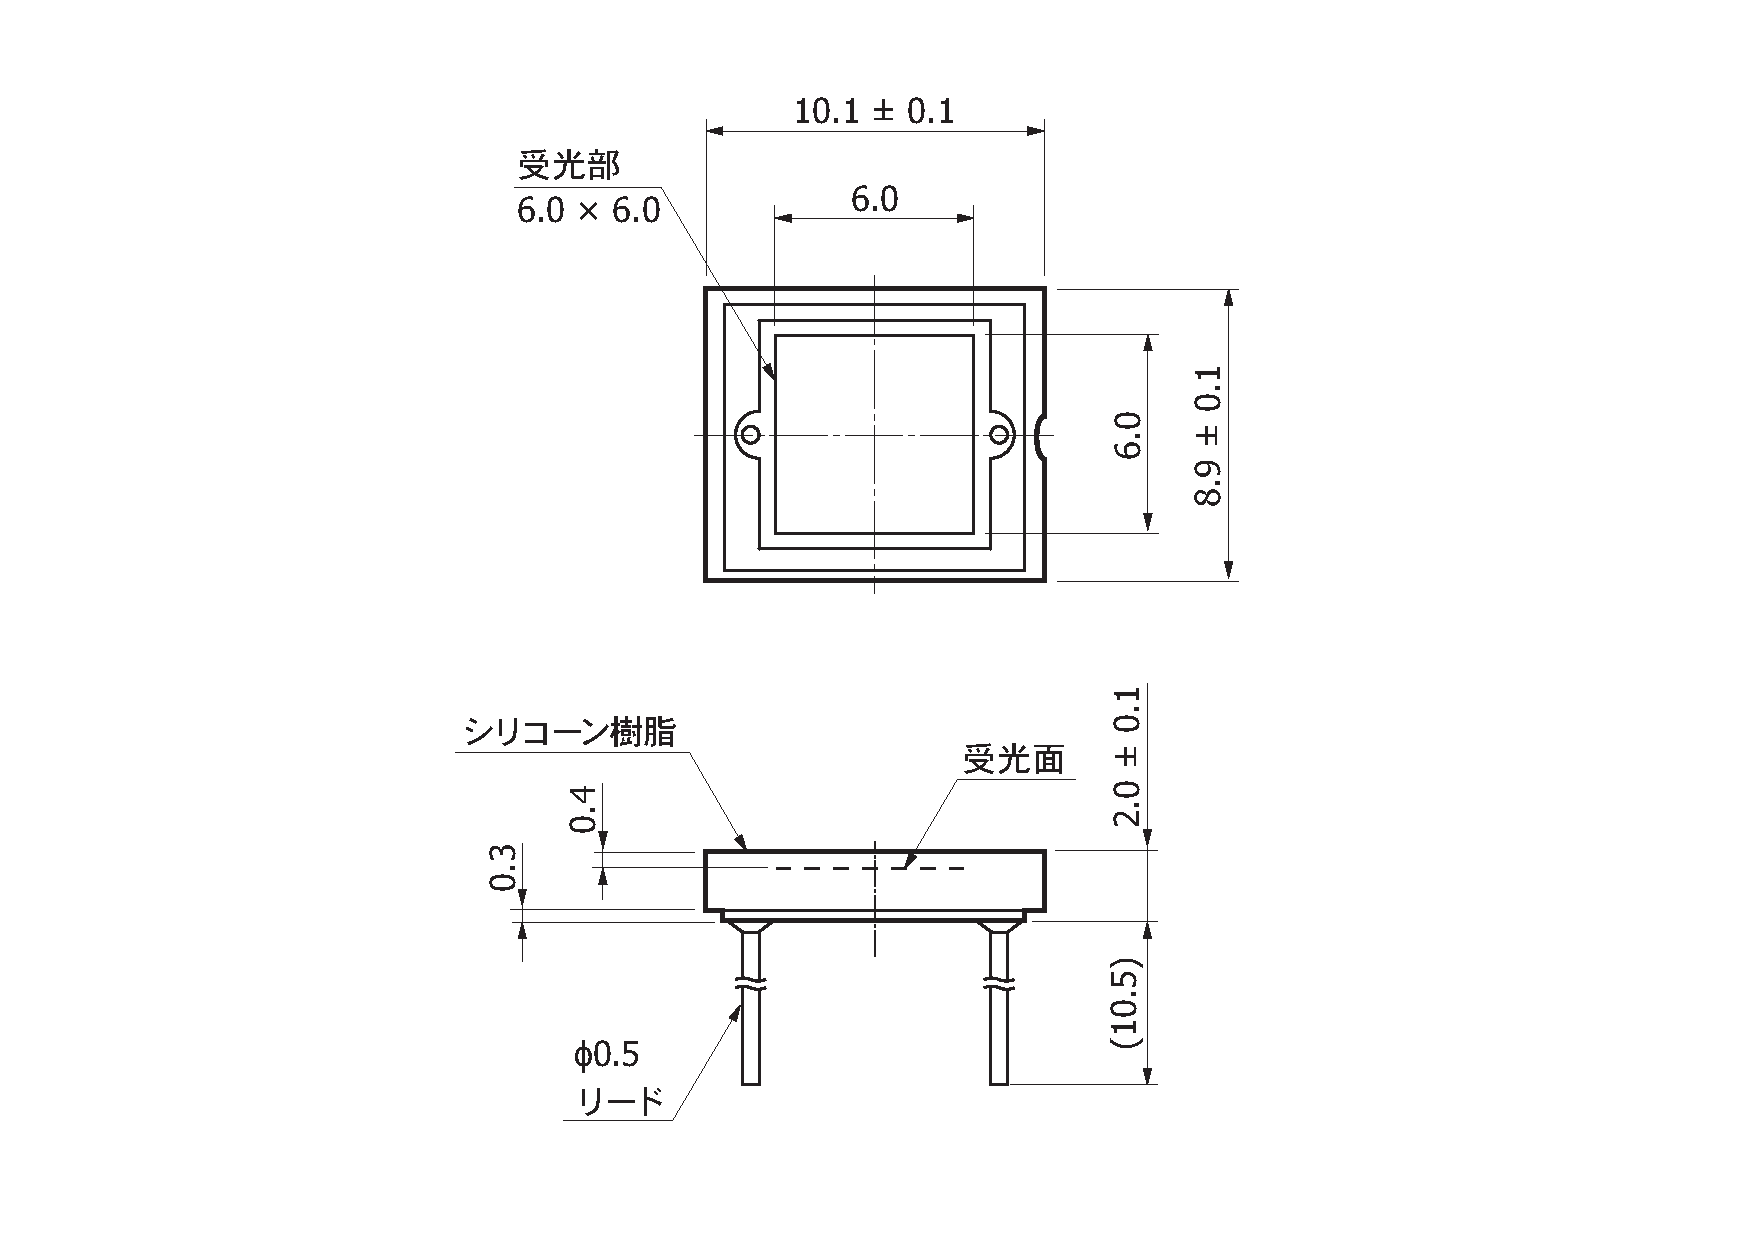
\includegraphics[width=15cm]{images/chapter4/MPPCshape.pdf}
  \caption{使用したMPPCの構造。。}
  \label{fig:MPPCshape}
\end{figure}

\subsection{コーン型ライトガイドのパラメータ}
第3章で求めたテスト実験でのMultiplicityを再現するように、コーン型ライトガイドの反射面の反射率を決定した。
シミュレーションで、コーン型ライトガイドの反射率を変化させていき、実験でのMultiplicityと一致する反射率を探した。
その際に、暗電流の影響はシミュレーションで自由に入れることができるため、
実験データのMultiplicityは十分ピークが入る$\SI{20}{ns}$のカット範囲での値を使用した。
シミュレーションにも$\SI{20}{ns}$分の暗電流を導入し、Multiplicityを確認した。
その結果を図\ref{fig:decideAl}に示す。

\begin{figure}
  \begin{tabular}{cc}
    \begin{minipage}{0.45\hsize}
      \centering
      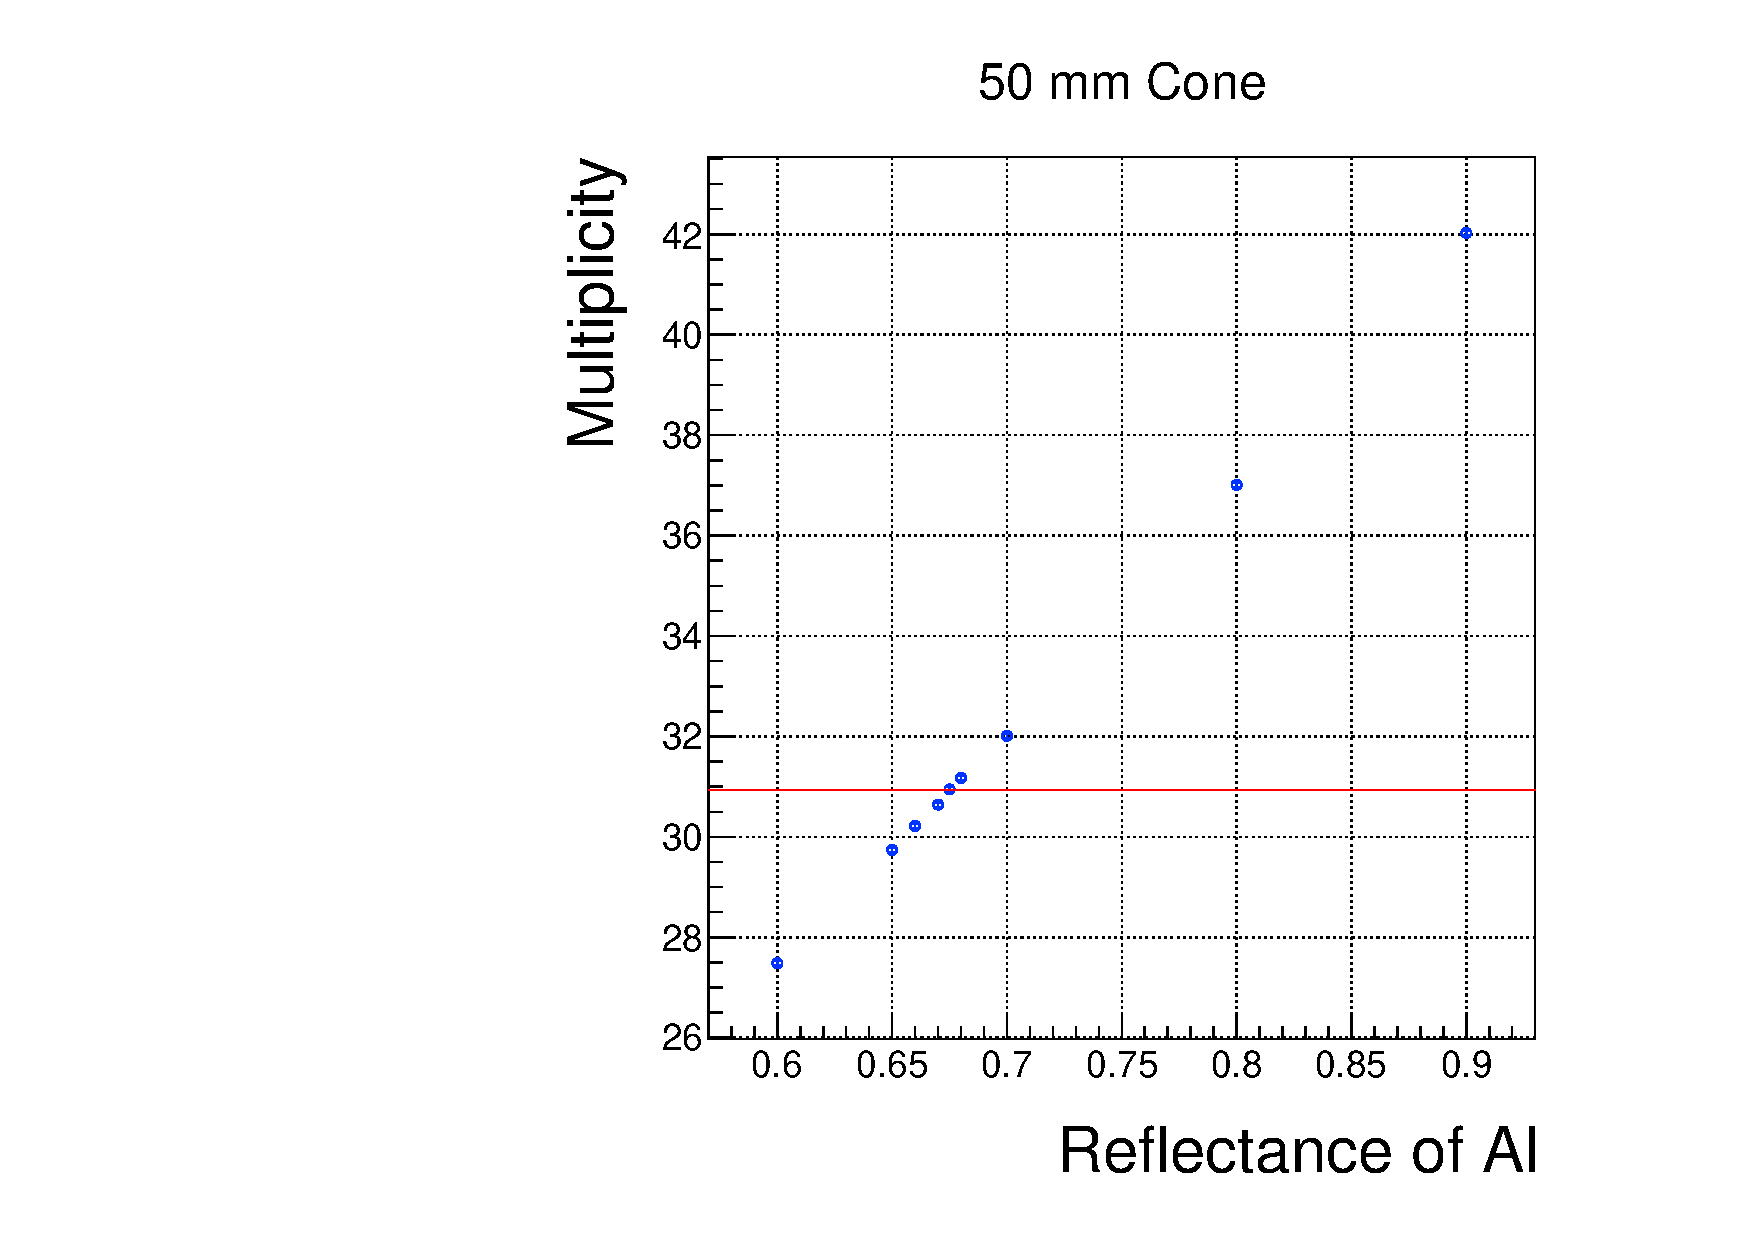
\includegraphics[keepaspectratio, scale=0.35, page=1]{images/chapter4/decideAl.pdf}
    \end{minipage} &
    \begin{minipage}{0.45\hsize}
      \centering
      \includegraphics[keepaspectratio, scale=0.35, page=2]{images/chapter4/decideAl.pdf}
    \end{minipage}
  \end{tabular}
  \caption{コーン反射面のアルミナイズドマイラーの最大反射率に対するMultiplicityの値。}
  \label{fig:decideAl}
\end{figure}

コーン反射面の反射率を、$\SI{50}{mm}$コーンでは0.675とした際に、$\SI{30}{mm}$コーンでは0.67とした際に実験データと一致した。
どちらのコーンでもほぼ等しい値が得られたことから、コーンの集光率低下の原因は反射面の影響であると考えられる。